\documentclass[12pt]{article}

\usepackage{xcolor}
\usepackage{listings}
\usepackage{hyperref}
\usepackage{pdfpages}

\hypersetup{
    colorlinks=true,
    linkcolor=blue,
    filecolor=magenta,      
    urlcolor=cyan,
    pdftitle={HW01},
    pdfpagemode=FullScreen,
    }
\lstset{basicstyle=\ttfamily,
showstringspaces=false,
commentstyle=\color{red},
keywordstyle=\color{blue}
}

\renewcommand{\thesubsection}{\thesection.\alph{subsection}}

\title{Programming Assignment 2 \\ \small{ECE 759, Prof. TW Huang}}
\author{Sai Tadinada}
\date{}

\begin{document}
\maketitle

GitHub link to programming tasks: \\ \url{https://github.com/phantom3012/repo759/tree/main/HW02}

\section{Question 1}
\subsection{}
scan.cpp can be found at \url{https://github.com/phantom3012/repo759/blob/main/HW02/scan.cpp}

\subsection{}
task1.cpp can be found at \url{https://github.com/phantom3012/repo759/blob/main/HW02/task1.cpp}

\subsection{}
Scaling analysis reveals an exponential increase in time starting from the point where the size of the array reachs $2^{24}$ elememts
\begin{figure}[ht]
    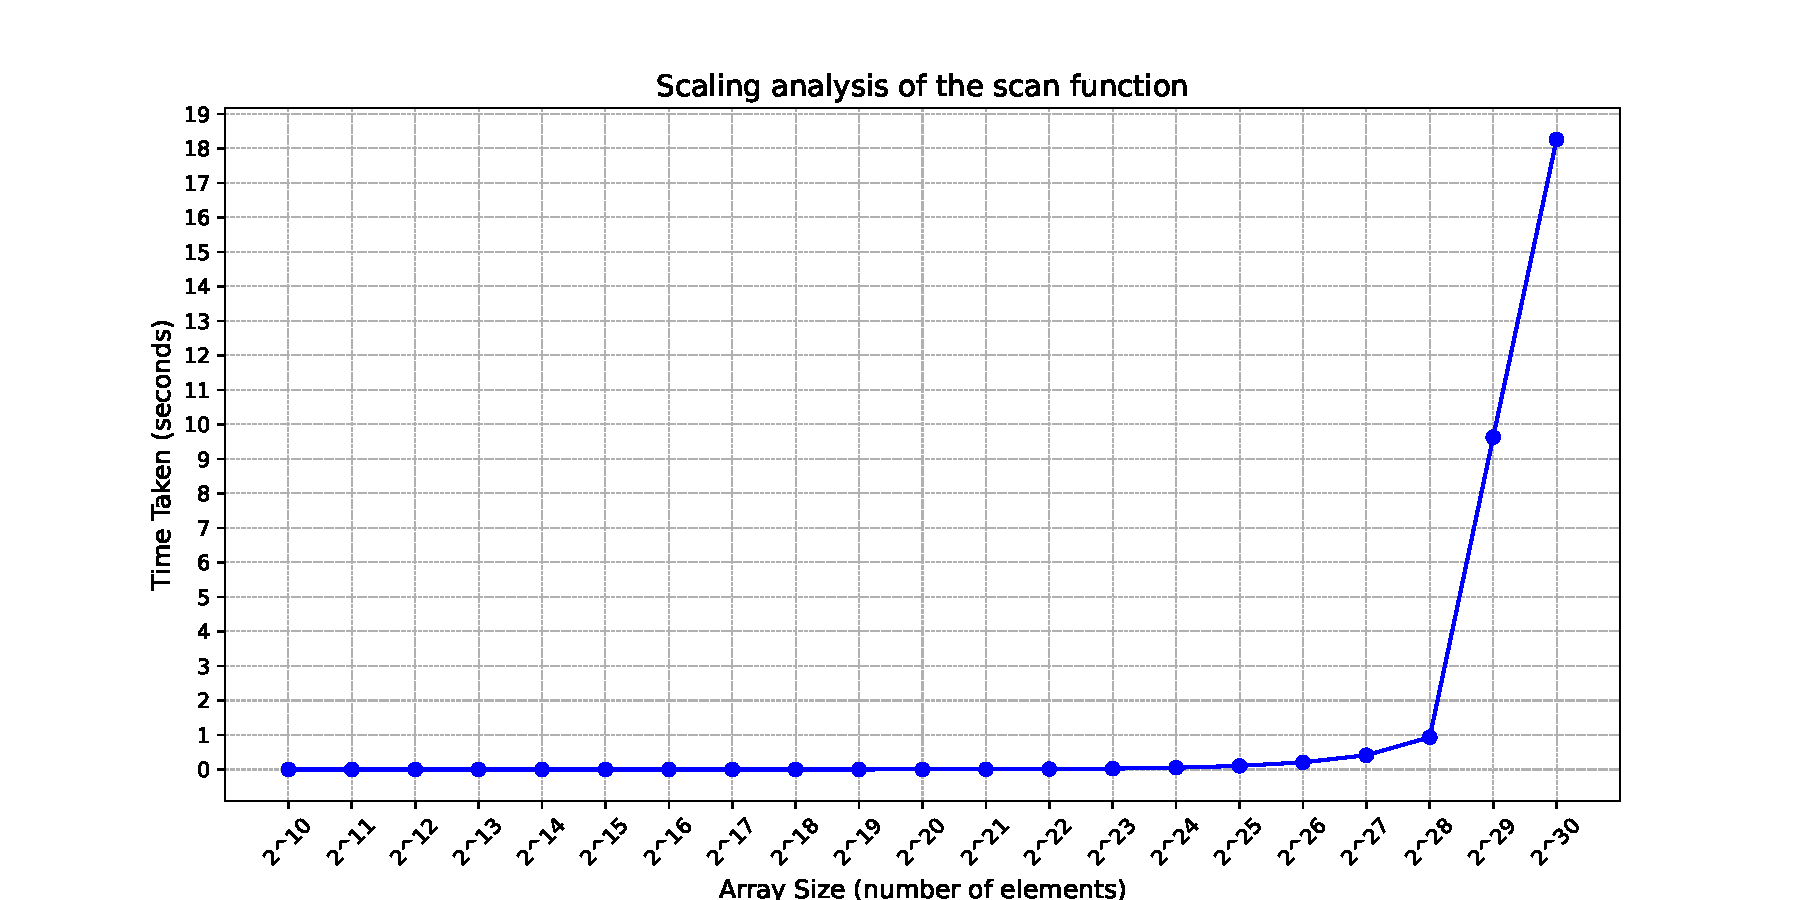
\includegraphics[width = \textwidth]{scan_scaling_analysis.pdf}
    \caption{Scaling analysis of scan.cpp}
\end{figure}

\section{Question 2}

\subsection{}
convolution.cpp can be found at \url{https://github.com/phantom3012/repo759/blob/main/HW02/convolution.cpp}
\subsection{}
task2.cpp can be found at \url{https://github.com/phantom3012/repo759/blob/main/HW02/task2.cpp}

\section{Question 3}
\subsection{}
Implementation of mmul1 can be found at \url{https://github.com/phantom3012/repo759/blob/main/HW02/matmul.cpp#L3}
\subsection{}
Implementation of mmul2 can be found at \url{https://github.com/phantom3012/repo759/blob/main/HW02/matmul.cpp#L13}
\subsection{}
Implementation of mmul3 can be found at \url{https://github.com/phantom3012/repo759/blob/main/HW02/matmul.cpp#L23}
\subsection{}
Implementation of mmul4 can be found at \url{https://github.com/phantom3012/repo759/blob/main/HW02/matmul.cpp#L33}
\subsection{}
task3.cpp can be found at \url{https://github.com/phantom3012/repo759/blob/main/HW02/task3.cpp}
\subsection{}
In ascending order of time taken, the functions can be arranged as follows: mmul2 $<$ mmul1 $\approx$ mmul4 $<$ mmul3\\ \\
mmul2 takes the least time because all accesses to all arrays are done in row-major form. In mmul1 and mmul4, the access to one operand is done in the column major form and in mmul3, all accesses are column major. This leads to a lot of cache misses and hence, the time taken is more. When accessed in row major, the time taken is significantly less (by almost a factor of 2) \\ \\
mmul4 and mmul1 take almost the same time. mmul4 on some instances may take slightly longer depending on the overheads posed by vector implementation.

\end{document}

